\documentclass{beamer}
\usepackage{ctex, hyperref}
\usepackage[T1]{fontenc}

% other packages
\usepackage{latexsym,amsmath,xcolor,multicol,booktabs,calligra}
\usepackage{graphicx,pstricks,listings,stackengine}
\usepackage{caption, subfigure}
\usepackage{listings}

% xmu beamer
\usepackage[blue]{TongjiBeamer}

\author[Wang Shixin]{王世鑫}
\title{FrenzyKV}
\subtitle{基于LSM存储引擎的NoSQL数据库管理系统}
\institute{德州学院计算机与信息学院}
\date{\today}


% defs6
\def\cmd#1{\texttt{\color{red}\footnotesize $\backslash$#1}}
\def\env#1{\texttt{\color{blue}\footnotesize #1}}

\lstset{
    basicstyle=\ttfamily\small,
    keywordstyle=\bfseries\color{red!0!green!0!blue!100},
    emphstyle=\ttfamily\color{red!100!green!0!blue!0},    % Custom highlighting style
    stringstyle=\color{red!0!green!100!blue!0},
    numbers=left,
    numberstyle=\small\color{gray!50},
    rulesepcolor=\color{red!20!green!20!blue!20},
    frame=shadowbox
}


\begin{document}
\begin{frame}
    \begin{figure}[htpb]
       \begin{center}
            \includegraphics[width=0.2\linewidth]{pic/DZU_logo.png}
        \end{center}
    \end{figure}
    \titlepage
\end{frame}

\begin{frame}
    \tableofcontents[sectionstyle=show,subsectionstyle=show/shaded/hide,subsubsectionstyle=show/shaded/hide]
\end{frame}

\section{本研究实现的功能概要}
\subsection{Koios 异步运行时}

\begin{frame}{异步运行时基本特点和功能}
	\begin{itemize}
        \item \textbf{基于 C++20 Coroutine}
        \item 基于 Linux IOUring 实现的高性能 Completion IO 模型
        \item \textbf{Work-Stealing 调度算法\cite{le_correct_nodate}}
        \item 可自定义事件循环
        \item 懒惰求值
        \item 高精度计时器 
        \item 协程异步运行时配套并发控制设施
        \begin{itemize}
            \item \textbf{异步队列化同步基类}
            \item 协程互斥锁
            \item 协程读写锁 
            \item \dots
        \end{itemize}
	\end{itemize}
\end{frame}

\begin{frame}{Work-Stealing Algorithm}
    \begin{figure}
        \centering
        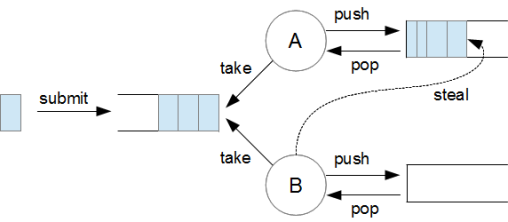
\includegraphics[width=0.8\linewidth]{pic/work_stealing.png}
        \caption{Work-Stealing 示意图}
    \end{figure}

    系统繁忙时,各工作线程处理各自任务,提高数据和指令局部性,缓存友好;
    系统闲时,空闲线程“偷取”忙线程任务,负载均衡。
\end{frame}

\subsection{Key-Value 存储}

\begin{frame}{存储基本功能和特点}
	\begin{itemize}
        \item 高性能异步IO\cite{crotty_are_2022}
        \item IO 4K Paging
        \item 基于 Skip-List\cite{pugh_skip_1990}的内存表
        \item \textbf{基于 SSTable\footnote{Sorted-String Table 排序字节串表} 的外存数据文件}
        \item 基于 Level 的LSM\cite{oneil_log-structured_1996}数据文件管理
        \item 冗余数据文件合并策略\footnote{Compacting and Merging Policy}
        \item \textbf{MVCC\footnote{Multi-Version Concurrency Control 多版本并发控制}}
        \item Bloom Filter\cite{burton_h_bloom_spacetime_1970}
        \item Snapshot Isolation\footnote{结合MVCC实现}
	\end{itemize}
\end{frame}

\begin{frame}{合并策略和文件结构}
    \begin{figure}
        \centering
        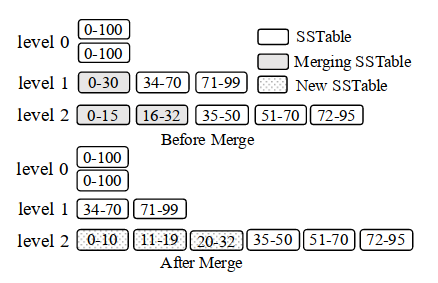
\includegraphics[width=0.8\linewidth]{pic/LSM_merging.png}
        \caption{合并策略示意图}
        %TODO
    \end{figure}
\end{frame}

\begin{frame}{合并策略和文件结构}
    \begin{figure}
        \centering
        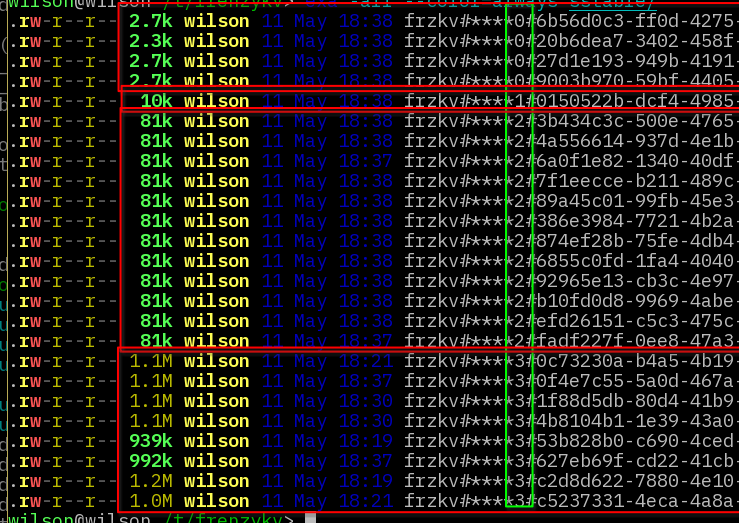
\includegraphics[width=0.9\linewidth]{pic/fs1.png}
        \caption{文件系统中测试文件示意图}
    \end{figure}
\end{frame}

\begin{frame}{合并策略和文件结构}
    \begin{figure}
        \centering
        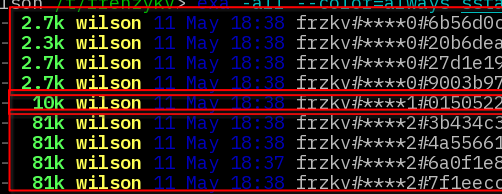
\includegraphics[width=0.9\linewidth]{pic/fs2.png}
        \caption{文件系统中测试文件示意图}
    \end{figure}
\end{frame}

\section{数据格式}

\begin{frame}{SSTable格式}
    \begin{figure}
        \centering
        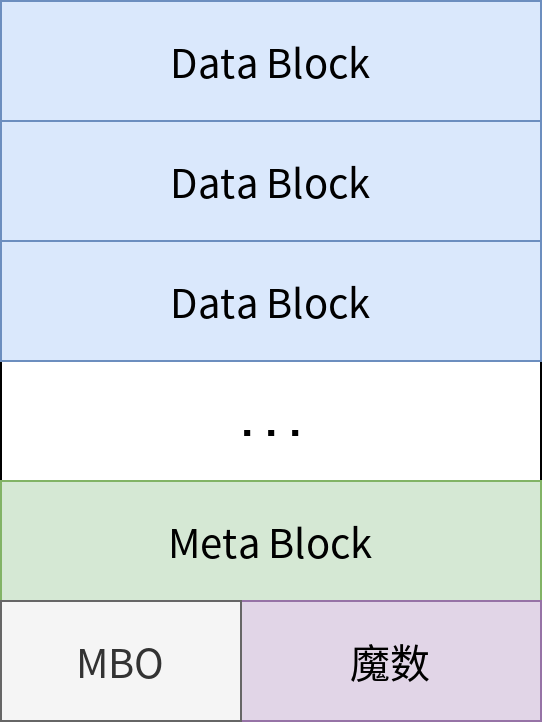
\includegraphics[width=0.3\linewidth]{pic/SSTable.png}
        \caption{SSTable格式}
    \end{figure}
    MBO: Meta Block Offset 元数据块偏移量
\end{frame}

\begin{frame}{块格式}
    \begin{figure}
        \centering
        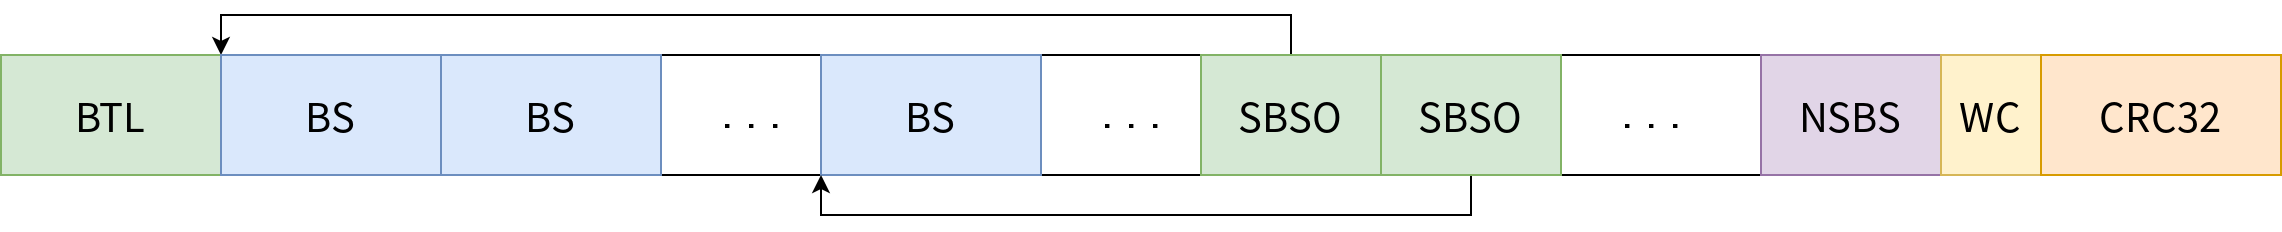
\includegraphics[width=1\linewidth]{pic/block.png}
        \caption{块格式}
    \end{figure}
    \begin{itemize}
        \item BTL: Block Total Length 整块长度
        \item BS: Block Segment 块内部段\footnote{每个内部段中数据具有公共前缀}
        \item SBSO: Special Block Segment Offsets 特殊块偏移量
        \item NSBS: 特殊块数量
        \item WC: Wether Compressed or not 是否压缩标志
        \item CRC32: 校验码
    \end{itemize}
\end{frame}

\begin{frame}{块内部段格式}
    \begin{figure}
        \centering
        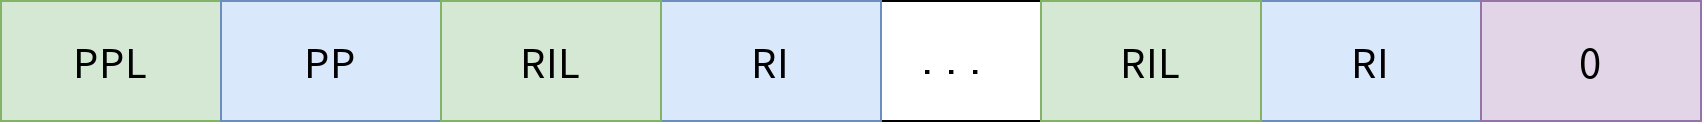
\includegraphics[width=1\linewidth]{pic/seg.png}
        \caption{块内部段格式}
    \end{figure}
    \begin{itemize}
        \item PPL: Public Prefix Length 公共前缀长度 
        \item PP: 公共前缀
        \item RIL: Rest Items Length 剩余元素长度
        \item RI: 剩余元素
        \item 末尾零\footnote{其长度和RIL相同} 表示当前段结束
    \end{itemize}
\end{frame}

\begin{frame}{键格式}
    \begin{figure}
        \centering
        
\includegraphics[width=0.8\linewidth]{pic/seqkey.png}
        \caption{序列键格式}
    \end{figure}
    键格式设计要点:
    \begin{itemize}
        \item 对象序列化前后比较结果相同 
        \item 具备相同用户键的记录,按照序列号排序.
    \end{itemize}
    本研究实现:
    \begin{itemize}
        \item 使用大端法表示整数
        \item 将序列号排在用户键后面
    \end{itemize}
\end{frame}

\begin{frame}{序列号是干什么用的}
    基于LSM结构数据文件不可变性,所有变化体现为新文件、新版本\footnote{参见第\ref{frm:mvcc}页}。
    因此对同一个Key可能有多个版本Value与之对应,需要使用一个序列号区分其出现先后次序。
\end{frame}

\section{MVCC 和快照隔离}

\begin{frame}{为什么要MVCC}\label{frm:mvcc}
    \begin{itemize}
        \item 快照隔离需要引用旧物理版本
        \item 实现读写互不干扰,实现高性能IO
    \end{itemize}
\end{frame}

\begin{frame}{文件管理应该做些什么?}
    为了\textbf{支持MVCC},本研究实现的文件管理组件具有以下特点:
    \begin{itemize}
        \item 文件名全局唯一\footnote{通过UUID}
        \item 系统运行期间维护对各个文件的引用计数\footnote{参见第\ref{frm:refcount}页}
        \item 条件触发或周期性触发过期\footnote{引用计数为0}文件GC
    \end{itemize}
\end{frame}

\begin{frame}{MVCC}
    每个版本持有若干数据文件的引用。
    此外,本研究实现的MVCC还有以下特点:
    \begin{itemize}
        \item 版本一旦创建,它引用的文件列表则不可修改\footnote{Immutable}
        \item 采用引用计数\footnote{快照会引用某版本}管理各版本生命期
        \item 各版本持有若干对数据文件的引用
        \item 新旧版本之间通过\textbf{版本差异}联系
        \item 新旧版本之间存在共享的文件也存在不共享的文件\footnote{快照隔离依托这一点实现}
    \end{itemize}

    版本差异通过包含:
    \begin{itemize}
        \item 相对上一个版本\textbf{移除}的文件
        \item 相对上一个版本\textbf{新增}的文件
    \end{itemize}
\end{frame}

\begin{frame}{版本差异}
    以下情况需相对上一版本\textbf{移除}文件:
    \begin{itemize}
        \item 该文件与其他文件被合并\footnote{Compacting and Merging}成一个新文件
        \item 全部内容为tombstones的文件被tombstones移除算法选中
    \end{itemize}

    \pause

    以下情况需相对上一版本\textbf{新增}文件:
    \begin{itemize}
        \item 新的内存表转换为SSTable刷入磁盘
        \item 从旧版本选中的若干文件合并出的新文件
    \end{itemize}
\end{frame}

\begin{frame}{如何构造新版本}

    \begin{equation*}
        L + \Delta = N
    \end{equation*}
    其中 $L$ 表示上一版本,$N$表示新版本。
    实际开发过程中也实现了类似的写法:
    \begin{figure}
        \centering
        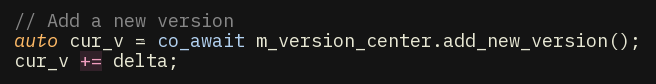
\includegraphics[width=0.8\linewidth]{pic/add-new-ver.png}
    \end{figure}
    在实现中,一旦出现新版本,上一版本的引用计数就会减1
\end{frame}

\begin{frame}{快照隔离}
    一个快照包含:
    \begin{itemize}
        \item 序列号
        \item 对某个版本的引用
    \end{itemize}
    各版本相对其他版本新增的文件互不可见,以此实现隔离。

    获取快照操作将会获取对当前版本的引用以及当前最大序列号。
    此后数据变化对此快照不可见。
\end{frame}

\section{其他技术细节}

\begin{frame}{在外存表中查找数据}
    \begin{figure}
        \centering
        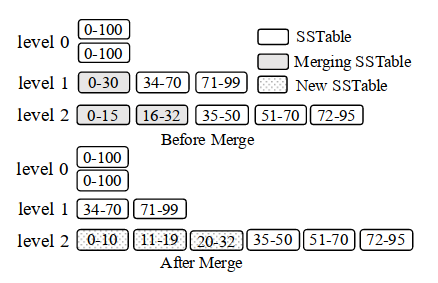
\includegraphics[width=0.8\linewidth]{pic/LSM_merging.png}
    \end{figure}

    从外存表中查找需要系统结合快照分别在
    $L_0, L_1, L_2, \dots$
    等级别文件中分别搜索目标键。
\end{frame}

\begin{frame}{Bloom Filter}
    布隆过滤器\cite{burton_h_bloom_spacetime_1970}
    是常用的数据库查询优化手段\cite{luo_lsm-based_2020}。

    优点:
    \begin{itemize}
        \item 体积小
        \item 基于\textit{多个}哈希函数实现,判定速度快
        \item 无\quad\textbf{不存在误报}\footnote{False Negative}
    \end{itemize}

    缺点:
    \begin{itemize}
        \item 长度不固定
        \item 低\quad\textbf{存在误报}率\footnote{
            False Positive Rate. 经测试,在特定情况下,
            本研究复现的Bloom Filter存在误报率低于$2\%$.
        }
    \end{itemize}
\end{frame}

\begin{frame}{Bloom Filter}
    本研究实现的过滤器对象接口具有以下功能
    \begin{itemize}
        \item 从多个Key构造
        \item 注册新Key
        \item 判定某Key是否在当前过滤器中注册
    \end{itemize}

    本研究复现的布隆过滤器基于\textit{MurMurHash 3 32-bits}算法实现。
\end{frame}

\begin{frame}{Bloom Filter}
    \begin{figure}
        \centering
        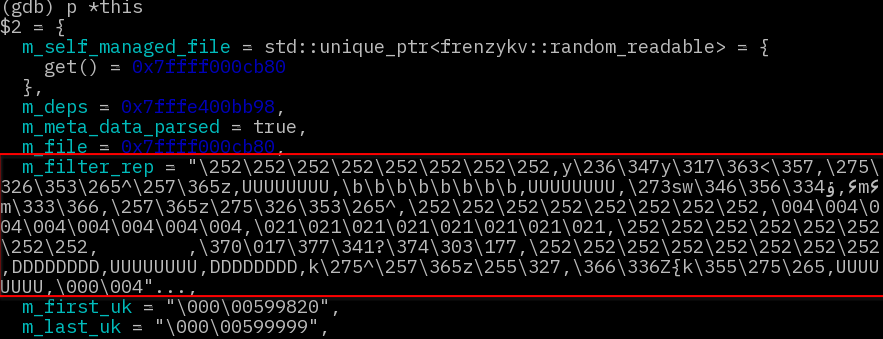
\includegraphics[width=0.9\linewidth]{pic/bloom-rep.png}
        \caption{布隆过滤器字节表示在GDB中的样子}
    \end{figure}
    过滤器在元数据块中,反序列化后可被SSTable对象直接访问
\end{frame}

\begin{frame}[fragile]{引用计数细节}\label{frm:refcount}
    \begin{minipage}{1\linewidth}
\begin{lstlisting}[language=C++]
auto fetch_add(::std::ptrdiff_t val = 1) noexcept
{
    return m_count.fetch_add(val, 
        ::std::memory_order_relaxed);
}

auto fetch_sub(::std::ptrdiff_t val = 1) noexcept
{
    return m_count.fetch_sub(val, 
        ::std::memory_order_acq_rel);
}
\end{lstlisting}
    \end{minipage}\hspace{1cm}
\end{frame}

\begin{frame}{Read Copy Update}
    \begin{figure}
        \centering
        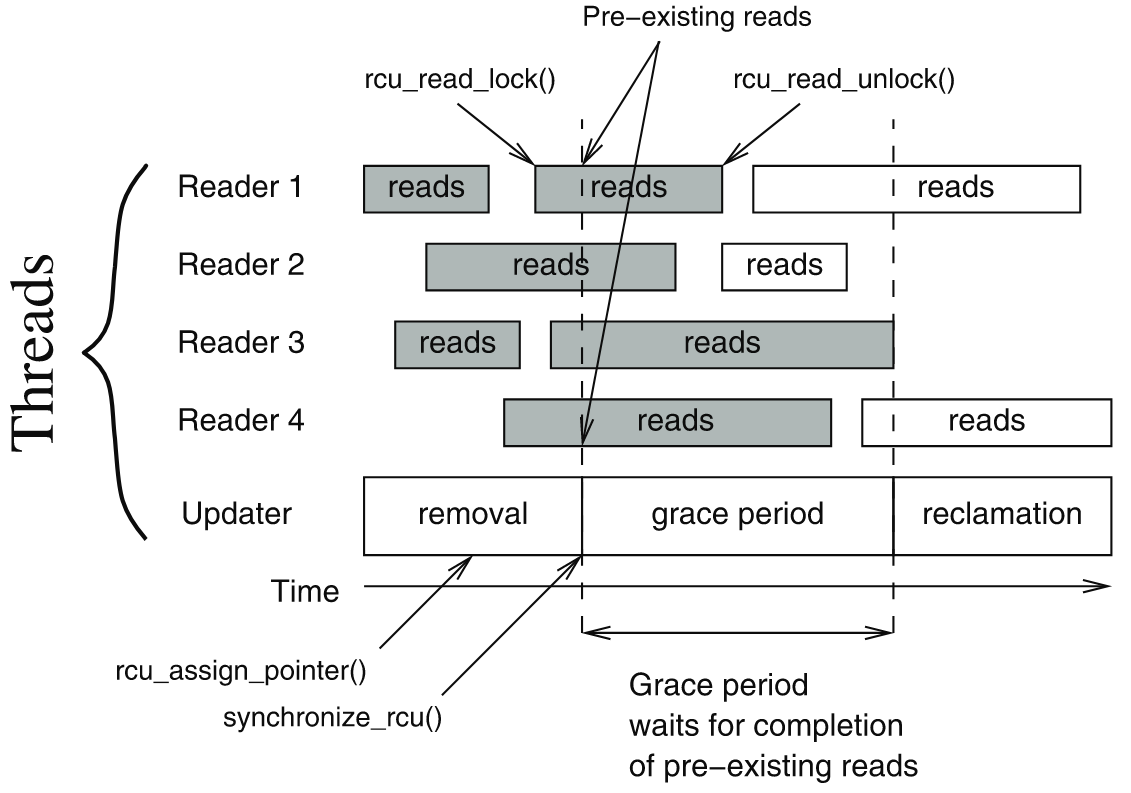
\includegraphics[width=0.6\linewidth]{pic/rcu.png}
        \caption{RCU操作示意图}
    \end{figure}
    RCU\cite{desnoyers_user-level_2011}
    在本研究中承担保存配置类以及环境信息等\textbf{多读少写}的信息
\end{frame}

\section{参考文献}

\begin{frame}[allowframebreaks]
    \bibliography{refe}
    %\bibliographystyle{alpha}
    % 如果参考文献太多的话,可以像下面这样调整字体:
    \tiny\bibliographystyle{alpha}
\end{frame}

\begin{frame}
    \begin{center}
        {\Huge\calligra Thanks!}
    \end{center}
\end{frame}

\end{document} 
